\section{Ejercicio 1}

\subsection{Inicializar la GDT}

Configuramos la GDT para tener bien configurada la segmentación al pasar a modo protegido.

Dejamos la primer entrada de la tabla vacía, por convención de la arquitectura, y las tres siguientes, que quedan reservadas para la práctica.

Además, creamos otras cinco entradas para nuestro uso:

\begin{itemize}
    \item Un segmento flat (con base 0 y límite de toda la memoria) de código con nivel de privilegio 0
    \item Un segmento flat de código con nivel de privilegio 3
    \item Un segmento flat de datos con nivel de privilegio 0
    \item Un segmento flat de datos con nivel de privilegio 3
    \item Un segmento de datos con nivel de privilegio 0, con base en $0xB8000$ y límite $80 * 50 * 2 - 1 = 7999 = 0x1F3F$
\end{itemize}

\subsection{Pasar a modo protegido}

Para pasar al modo protegido debemos habilitar primero A20 con la rutina provista por la cátedra, luego cargar la GDT con la instrucción $LGDT$, habilitar el bit PE del registro CR0 que setea el modo protegido propiamente dicho, y saltar a una sección del código programada en 32 bits.

\begin{lstlisting}
    ; Habilitar A20
    call habilitar_A20

    ; Cargar la GDT
    lgdt [GDT_DESC]

    ; Setear el bit PE del registro CR0
    mov eax, cr0
    or eax, 1
    mov cr0, eax

    ; Saltar a modo protegido
    jmp GDT_CODE_0_DESC:mp
\end{lstlisting}

\subsection{Imprimir el mapa inicial}

La memoria de video que mapeamos anteriormente representa un mapa de caracteres de 80 columnas y 50 líneas, con cada caracter representado como un byte con su valor ASCII y un byte con sus atributos (color de letra, color de fondo y un flag de blink).

Para inicializar el mapa recorremos el array y escribimos los valores que queremos para obtener la figura \ref{fig:mapa-inicial}

\begin{figure}[H]
    \centering
    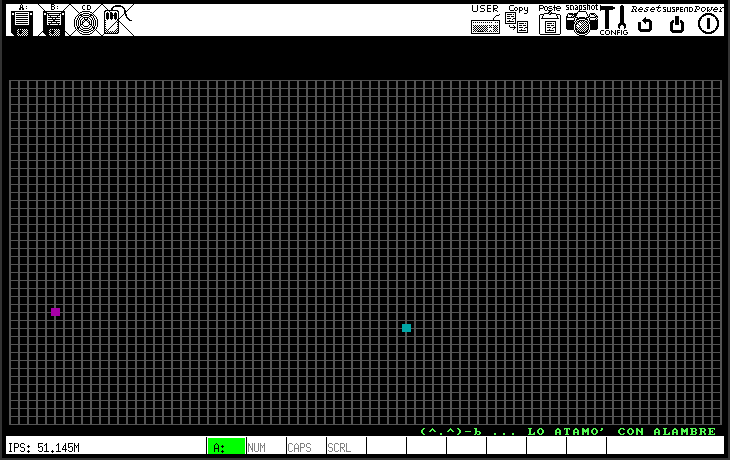
\includegraphics[width=\textwidth]{mapa-inicial}
    \caption{Mapa inicial}
    \label{fig:mapa-inicial}
\end{figure}

